\documentclass[conference]{IEEEtran}
\IEEEoverridecommandlockouts

\usepackage{cite}
\usepackage{amsmath,amssymb,amsfonts}
\usepackage{algorithmic}
\usepackage{graphicx}
\usepackage{textcomp}
\usepackage{xcolor}
\usepackage{booktabs}
\usepackage{multirow}
\usepackage{hyperref}

\def\BibTeX{{\rm B\kern-.05em{\sc i\kern-.025em b}\kern-.08em
    T\kern-.1667em\lower.7ex\hbox{E}\kern-.125emX}}

\begin{document}

\title{Machine Learning-Driven Biological Age Estimation and Survival Risk Stratification Using Routine Blood Biomarkers}

\author{\IEEEauthorblockN{Davinder Paul Singh\IEEEauthorrefmark{1},
Prutha Thakkar\IEEEauthorrefmark{1},
Sargam Malaviya\IEEEauthorrefmark{1},
Pawandeep Kour\IEEEauthorrefmark{2},
Shubham Mahajan\IEEEauthorrefmark{3}, and
Debabrata Swain\IEEEauthorrefmark{1}}
\IEEEauthorblockA{\IEEEauthorrefmark{1}Department of Computer Science and Engineering, Pandit Deendayal Energy University, Gandhinagar, Gujarat, India\\
Email: \{davinder.singh, prutha.tce21, sargam.mce21, debabrata.swain\}@sot.pdpu.ac.in}
\IEEEauthorblockA{\IEEEauthorrefmark{2}Department of Chemistry, University of Kashmir, Srinagar, Jammu and Kashmir, India\\
Email: pkour5400@gmail.com}
\IEEEauthorblockA{\IEEEauthorrefmark{3}Amity School of Engineering and Technology, Amity University, Panchgaon, Haryana, India\\
Email: mahajanshubham2232579@gmail.com}}

\maketitle

\begin{abstract}
Chronological age measures elapsed calendar time but inherently fails to capture inter-individual variation in multi-system physiological decline. This study introduces an end-to-end machine learning framework to estimate biological age from a panel of 12 standard clinical and blood chemistry biomarkers, and evaluates whether algorithmic biological age acceleration independently predicts long-term all-cause mortality risk. Leveraging the NHANES IV multi-cycle cohort ($N = 35,723$ adult participants; longitudinal follow-up $N = 26,425$ with 2,181 mortality events over a median 116.0 person-months), we benchmark six supervised learning architectures under strict leakage-free partitioning and five-fold cross-validation. In Experiment A (incorporating chronological age with biomarkers), our Multilayer Perceptron (MLP) achieves superior estimation accuracy with a holdout Mean Absolute Error (MAE) of 2.8401 years, Root Mean Squared Error (RMSE) of 3.8643 years, $R^2$ of 0.9640, and Pearson $r$ of 0.9819, closely rivaled by XGBoost (RMSE: 3.9122 years). In Experiment B (biomarkers only), models isolate pure somatic aging signals, accounting for 68.86\% of phenotypic variance without chronological input. Longitudinal survival modeling demonstrates that biological age acceleration conveys marked prognostic divergence (Log-Rank $\chi^2 = 625.76, p < 0.0001$). Multivariable Cox proportional hazards modeling demonstrates that each additional year of biological age acceleration confers an independent 6.78\% increase in all-cause mortality hazard ($\text{HR} = 1.0678$, 95\% CI: 1.0516--1.0842, $p < 0.0001$), even after adjusting for chronological age. These findings establish that supervised learning models trained on routine clinical blood chemistry can effectively measure physiological aging and provide robust prognostic clinical decision support.
\end{abstract}

\begin{IEEEkeywords}
Biological age estimation, Machine learning, Phenotypic aging, Blood biomarkers, Survival analysis, Cox proportional hazards, Explainable AI.
\end{IEEEkeywords}

\section{Introduction}
Aging is a progressive, multi-faceted decline in physiological reserve, molecular repair capacity, and homeostatic resilience occurring across all biological systems \cite{lopez2013hallmarks}. While chronological age---the duration elapsed since birth---is ubiquitously employed in clinical practice as the primary benchmark for disease vulnerability and risk stratification, it fails to account for the marked heterogeneity in individual rates of somatic senescence \cite{crimmins2008biomarkers}. Two individuals of identical chronological age frequently display strikingly disparate physiological profiles; one may retain robust cardiovascular, metabolic, and renal vitality, whereas the other exhibits multi-system vulnerability, chronic subclinical inflammation, and premature organ decay.

This marked divergence has established the clinical construct of \textit{biological age}---an objective, scalar reflection of an organism's functional integrity relative to population baselines \cite{belsky2015quantification}. The difference between biological age and chronological age, termed \textit{biological age acceleration} ($\Delta = \text{Predicted BioAge} - \text{Chronological Age}$), serves as an actionable metric: individuals with positive acceleration ($\Delta > 0$) age at an elevated physiological velocity and carry heightened risks of age-related morbidity and premature mortality \cite{levine2018epigenetic}.

While molecular epigenetic clocks based on DNA methylation (such as Horvath and GrimAge clocks \cite{horvath2013dna, lu2019dna}) offer valuable insights into cellular mitotic turnover, their high cost, complex assay workflows, and specialized sequencing requirements severely impede their translation into everyday clinical practice. Conversely, routine clinical and blood chemistry panels---such as liver enzymes, creatinine, glycated hemoglobin, lipids, and leukocyte differentials---are routinely ordered during annual medical checkups at minimal cost. Synthesizing these standard blood analytes into an accurate, reproducible biological age estimate represents a significant opportunity for proactive preventive medicine and automated clinical decision support \cite{zhavoronkov2019deep}.

Conventional biomarker aging algorithms, such as the Klemera-Doubal Method (KDM) \cite{klemera2006new} and PhenoAge \cite{levine2018epigenetic}, rely on linear equations or parametric survival regressions. However, human physiological systems are governed by non-linear compensatory interactions, threshold phenomena, and multi-organ feedback loops that parametric models struggle to represent. Modern supervised learning algorithms, including tree-based gradient boosting and deep artificial neural networks, provide an optimal inductive mechanism to capture these non-linear multi-analyte dynamics.

This study presents three primary contributions:
\begin{itemize}
    \item \textbf{End-to-End Leakage-Free ML Architecture:} We formulate a robust, leakage-free pipeline evaluating six distinct machine learning architectures across 35,723 adult participants from the continuous NHANES IV database, establishing standardized regression benchmarks.
    \item \textbf{Controlled Decoupling Analysis:} Through dual experimental configurations (Experiment A with chronological age vs. Experiment B without), we rigorously decouple calendar time anchoring from pure biological aging signals, revealing that blood biomarkers alone account for 68.86\% of phenotypic variance.
    \item \textbf{Longitudinal Prognostic Validation:} Using an embedded survival cohort of 26,425 individuals followed for up to 201 months (2,181 mortality events), we validate that algorithmic biological age acceleration independently predicts all-cause mortality hazard ($\text{HR} = 1.0678, p < 0.0001$), outperforming traditional baseline formulations.
\end{itemize}

\section{Literature Survey}
Quantitative biogerontology has evolved through distinct conceptual methodologies over the past two decades. Early attempts to model biological aging centered on multiple linear regression, in which biomarkers were regressed against chronological age. However, this approach suffered from fundamental regression-to-the-mean artifacts and conceptual circularity, as it forced predicted biological age to mimic calendar time rather than independent physiological vulnerability \cite{nakamura1988assessment}.

To address these limitations, Klemera and Doubal (2006) formulated the Klemera-Doubal Method (KDM) \cite{klemera2006new}, which treats chronological age and physiological decline as latent variables within an inverse regression framework. While mathematically elegant, KDM presupposes linear relationships between biomarkers and age and treats biomarkers as statistically independent, an assumption violated by the interconnected nature of renal, cardiovascular, and metabolic regulatory networks \cite{cohen2015statistical}.

A transformative advance occurred in 2018 when Levine et al. developed the \textit{Phenotypic Age} (PhenoAge) algorithm \cite{levine2018epigenetic}. Rather than calibrating biomarkers against chronological age, Levine et al. calibrated an elastic-net penalized Gompertz proportional hazards model on mortality risk within the third National Health and Nutrition Examination Survey (NHANES III). Ten parameters (chronological age plus nine clinical blood analytes) were selected based on mortality prognostic power and converted into a phenotypic biological age scale. Kwon et al. (2021) expanded this work by developing the R package \textit{BioAge} \cite{kwon2021bioage}, which standardized PhenoAge, KDM, and homeostatic dysregulation metrics across continuous NHANES cohorts. We utilize the BioAge PhenoAge definition as an established clinical benchmark while developing an independent, non-linear machine learning and survival framework.

In recent years, deep learning and tree-based ensemble methods have achieved breakthrough performance in medical diagnostics \cite{chen2016xgboost, lundberg2017unified}. However, prior applications of machine learning to blood biomarker aging clocks have frequently suffered from critical methodological flaws: (i) data leakage caused by fitting normalizers and imputers across the entire dataset prior to partitioning; (ii) lack of comprehensive multi-model benchmarking across deep neural networks, kernel machines, and tree ensembles; and (iii) failure to isolate chronological age leakage from intrinsic biomarker predictive capacity \cite{pyrkov2018quantitative}. Our work directly resolves these limitations through a leak-free protocol, rigorous out-of-sample benchmarking, SHAP-based feature attribution, and longitudinal survival evaluation.

\section{Methodology}

\subsection{Dataset Collection and Cohort Provenance}
The empirical foundation of this study is drawn from the continuous National Health and Nutrition Examination Survey (NHANES IV, 1999--2018), accessed via the BioAge repository \cite{kwon2021bioage}. The uncurated NHANES IV dataset comprises 55,081 participant records across 89 demographic, examination, and laboratory variables. NHANES employs a complex, stratified, multistage probability cluster sampling design representative of the non-institutionalized civilian United States population.

To ensure analytical rigor and eliminate synthetic noise from artificial imputation, we enforced strict complete-case verification across 13 candidate physiological features and the phenotypic biological age target (\texttt{phenoage0}). Filtering complete cases yielded an analytic cohort of \textbf{35,723 adult participants} (mean chronological age: $49.61 \pm 18.27$ years, range: 20.0--85.0; mean PhenoAge: $46.78 \pm 20.19$ years, range: 4.24--115.29). Embedded within this cohort is a longitudinal surveillance subset of \textbf{26,425 individuals} with verified mortality linkage via the National Death Index (NDI), recording 2,181 all-cause deaths across a median follow-up of 116.0 person-months (maximum: 201.0 months).

\subsection{Data Preprocessing and Leakage-Free Scaling}
To ensure clinical relevance and prevent numerical instability during gradient backpropagation, right-skewed inflammatory and renal biomarkers were log-transformed: natural log C-reactive protein ($\text{lncrp} = \ln(\text{CRP}, \text{mg/dL})$) and natural log serum creatinine ($\text{lncreat\_umol} = \ln(\text{Creatinine}, \mu\text{mol/L})$). All continuous features were standardized using z-score normalization:
\begin{equation}
z_{ij} = \frac{x_{ij} - \mu_j}{\sigma_j}
\end{equation}

\textbf{Zero-Leakage Guarantee:} A critical vulnerability in published biomedical ML pipelines is fitting scalers on the entire dataset before partitioning, which leaks test-set distributional parameters into the training phase. In our pipeline, all normalization parameters $(\mu_j, \sigma_j)$ are computed strictly on the training partition and then applied downstream to transform unseen test folds without retraining.

\subsection{Feature Space and Physiological Domains}
The feature space consists of 13 routine clinical indicators spanning six key physiological organ systems:
\begin{itemize}
    \item \textbf{Macro-Temporal Anchor:} Chronological Age (\texttt{age}, years).
    \item \textbf{Metabolic \& Glycemic Regulation:} Glycated Hemoglobin (\texttt{hba1c}, \%), Total Cholesterol (\texttt{totchol}, mg/dL).
    \item \textbf{Renal Filtration \& Clearance:} Log Serum Creatinine (\texttt{lncreat\_umol}, $\ln(\mu\text{mol/L})$), Blood Urea Nitrogen (\texttt{bun}, mg/dL), Serum Uric Acid (\texttt{uap}, mg/dL).
    \item \textbf{Hepatic Function \& Nutrition:} Serum Albumin (\texttt{albumin\_gL}, g/L), Alkaline Phosphatase (\texttt{alp}, U/L).
    \item \textbf{Sterile Systemic Inflammation:} Log C-Reactive Protein (\texttt{lncrp}, $\ln(\text{mg/dL})$), White Blood Cell Count (\texttt{wbc}, $10^3/\mu\text{L}$).
    \item \textbf{Hematology \& Hemodynamics:} Lymphocyte Percentage (\texttt{lymph}, \%), Mean Corpuscular Volume (\texttt{mcv}, fL), Systolic Blood Pressure (\texttt{sbp}, mmHg).
\end{itemize}

\subsection{Data Partitioning and Cross-Validation Protocol}
To guarantee unbiased evaluation, the cohort was partitioned into an 80\% training set ($N = 28,578$) and a 20\% holdout test set ($N = 7,145$) using fixed pseudorandom initialization ($\text{seed} = 42$). Row indices were serialized (\texttt{train\_indices.npy}, \texttt{test\_indices.npy}) to ensure complete reproducibility. Within the training fold, 5-fold cross-validation was conducted across all candidate models to tune hyperparameters and check generalization stability. The holdout test set was sequestered and evaluated only after model training and parameter freezing was complete.

\subsection{Experimental Configurations}
To isolate the predictive contributions of chronological age versus blood chemistry, two distinct experiments were executed:
\begin{itemize}
    \item \textbf{Experiment A (Age + 12 Biomarkers, $d=13$):} Evaluates real-world clinical estimation where patient calendar age is known alongside routine laboratory results.
    \item \textbf{Experiment B (12 Biomarkers Only, $d=12$):} Chronological age is completely removed from the input matrix, forcing models to estimate physiological status purely from biochemical indicators.
\end{itemize}

\subsection{Candidate Learning Architectures}
We benchmarked six diverse regression paradigms: (1) Ordinary Least Squares (OLS) baseline; (2) Random Forest Regressor (100 estimators, max depth 12); (3) Support Vector Regressor (SVR with RBF kernel, $C=10.0, \epsilon=0.1$); (4) Gradient Boosting Machine (100 estimators, learning rate 0.1); (5) Extreme Gradient Boosting (XGBoost, max depth 6, eta 0.08, subsample 0.85); and (6) Multilayer Perceptron (MLP, 3 hidden layers: $128 \to 64 \to 32$ units, ReLU activation, batch size 64, Adam optimizer, early stopping).

\begin{figure}[t]
\centering
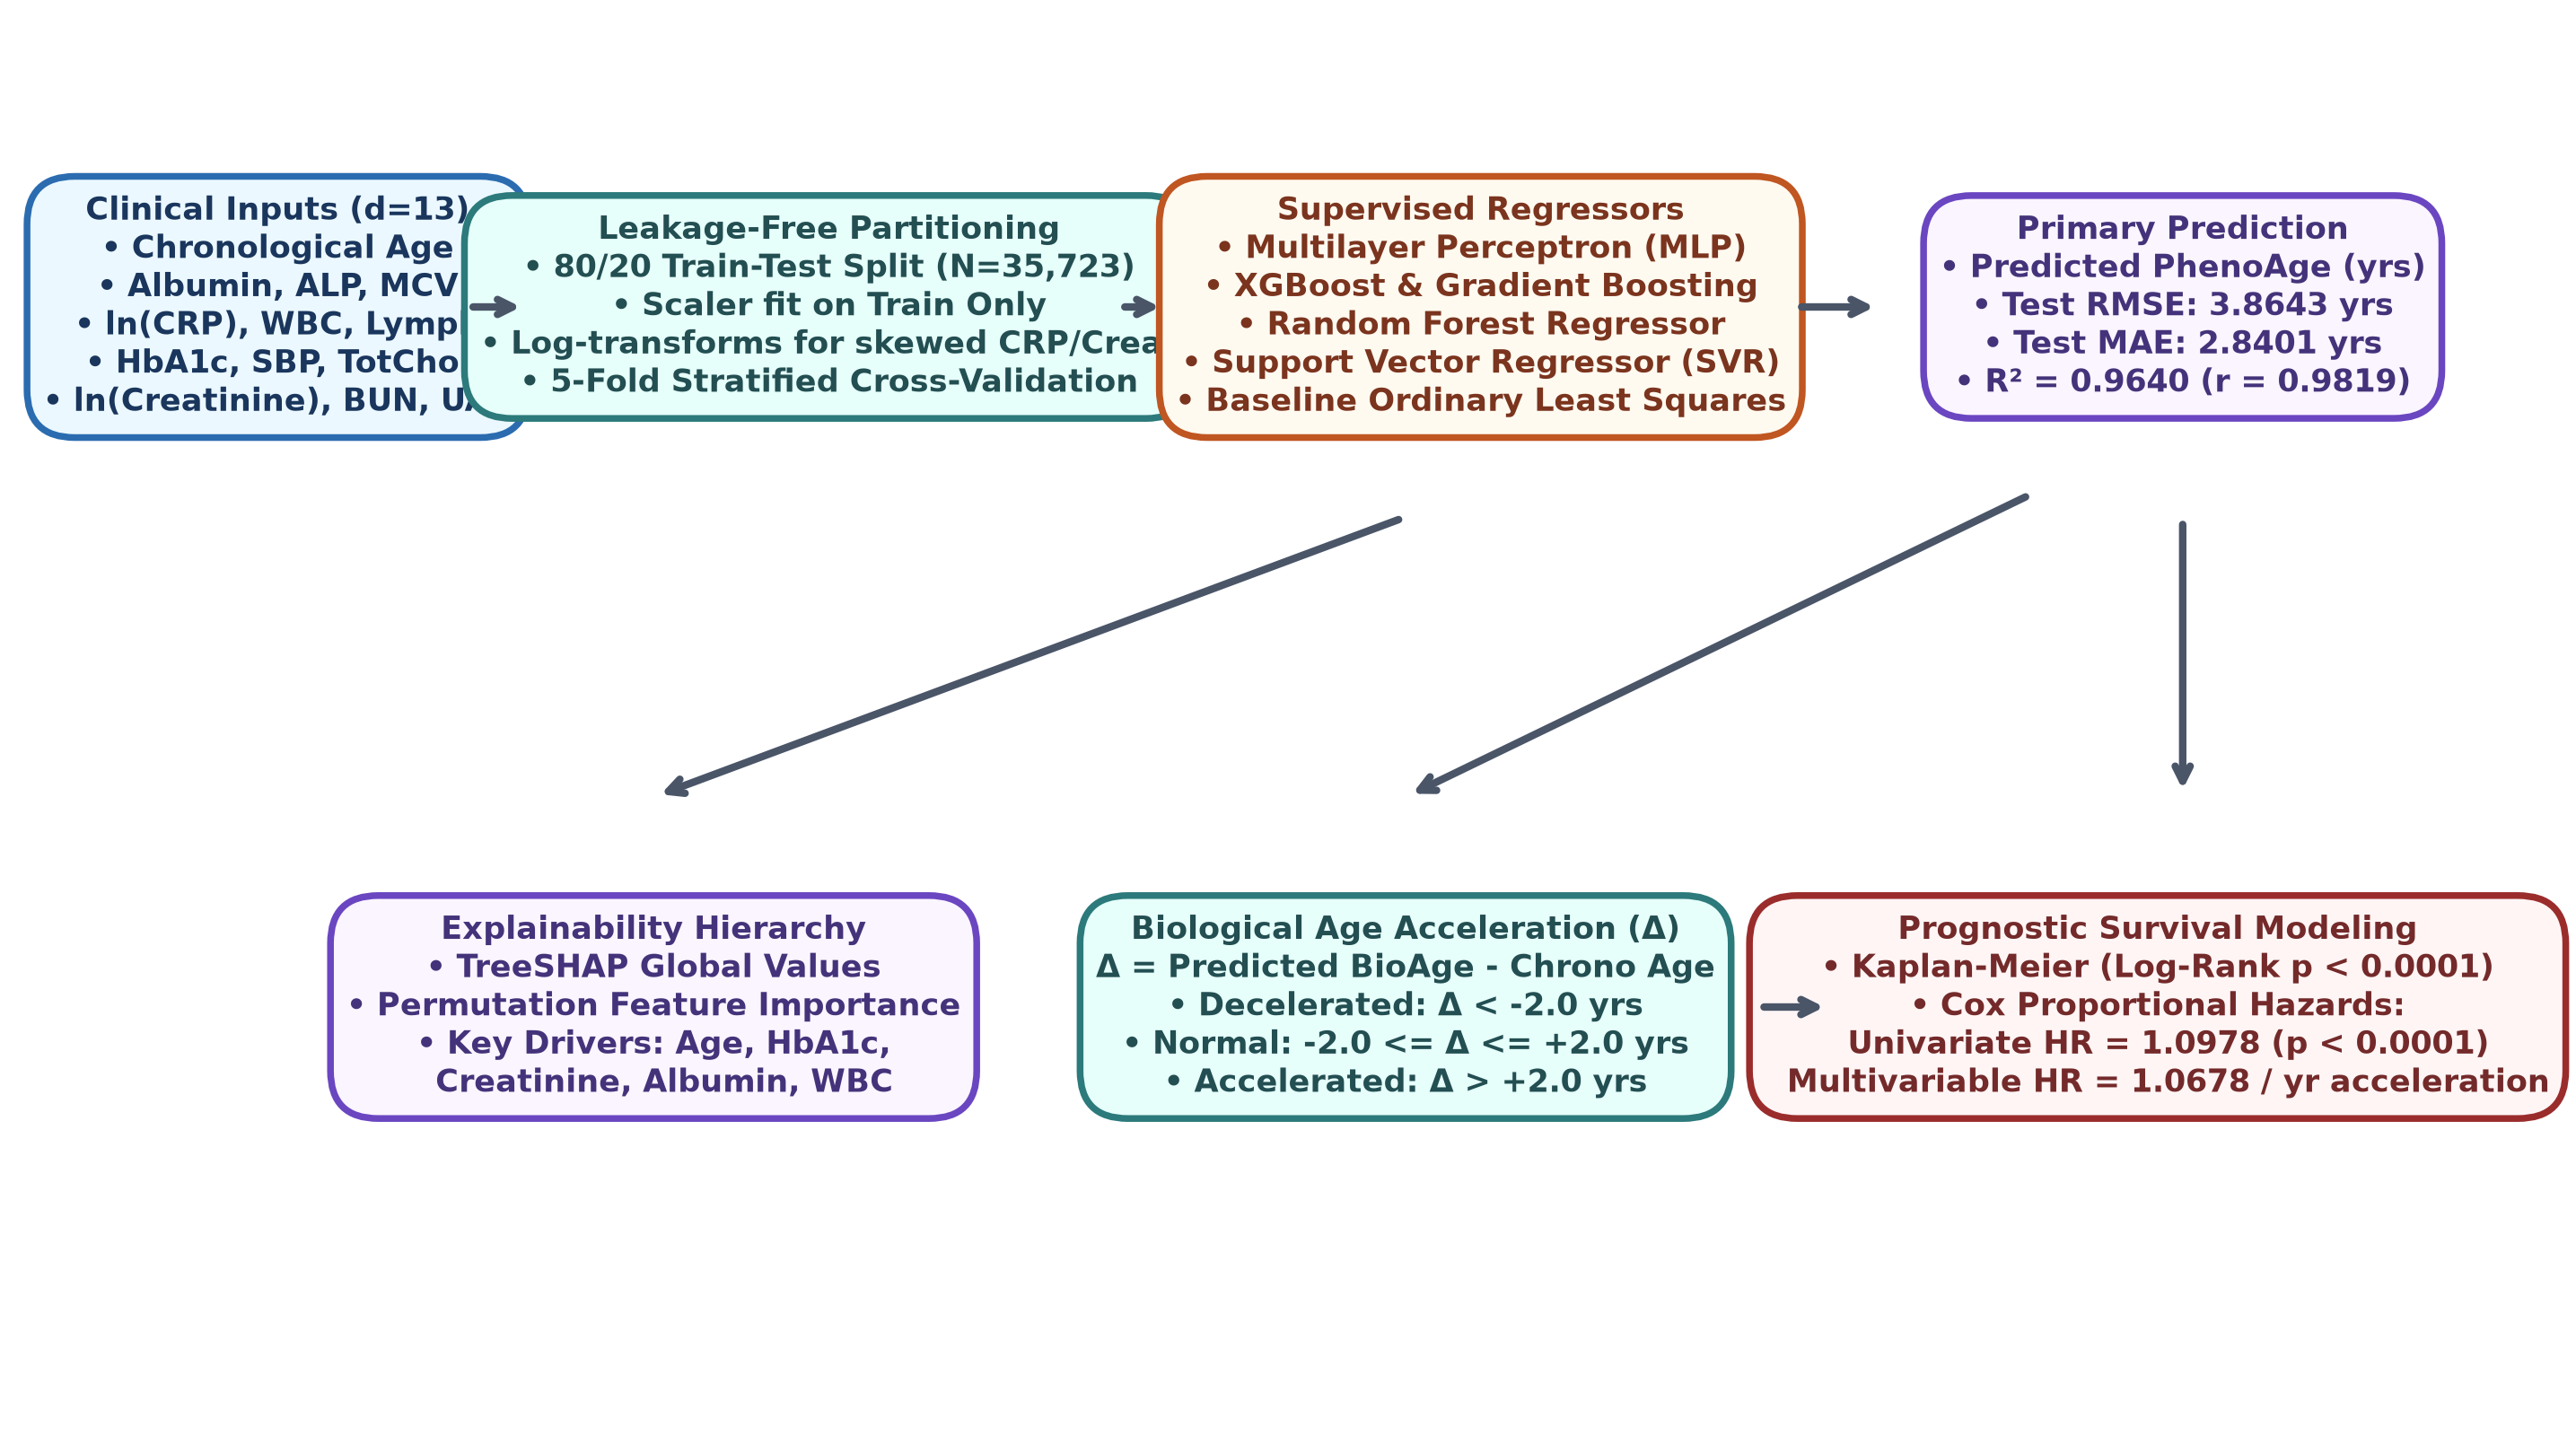
\includegraphics[width=\linewidth]{results/figures/architecture_diagram.png}
\caption{End-to-end system architecture: from routine clinical biomarker inputs through leakage-free preprocessing, multi-model regression benchmarking, SHAP explainability, and downstream longitudinal survival analysis.}
\label{fig:arch}
\end{figure}

\section{Evaluation Metrics}
Model performance on the holdout test set was evaluated across five complementary statistical regression metrics:

\begin{itemize}
    \item \textbf{Mean Absolute Error (MAE):} Quantifies average magnitude of prediction error in years:
    \begin{equation}
    \text{MAE} = \frac{1}{N} \sum_{i=1}^N |y_i - \hat{y}_i|
    \end{equation}
    \item \textbf{Root Mean Squared Error (RMSE):} Penalizes large individual deviations:
    \begin{equation}
    \text{RMSE} = \sqrt{\frac{1}{N} \sum_{i=1}^N (y_i - \hat{y}_i)^2}
    \end{equation}
    \item \textbf{Coefficient of Determination ($R^2$):} Fraction of target variance explained:
    \begin{equation}
    R^2 = 1 - \frac{\sum_{i=1}^N (y_i - \hat{y}_i)^2}{\sum_{i=1}^N (y_i - \bar{y})^2}
    \end{equation}
    \item \textbf{Pearson Correlation ($r$) and Spearman Rank ($\rho$):} Assess parametric linearity and monotonic rank-order concordance:
    \begin{equation}
    r = \frac{\text{Cov}(y, \hat{y})}{\sigma_y \sigma_{\hat{y}}}, \quad \rho = 1 - \frac{6 \sum d_i^2}{N(N^2 - 1)}
    \end{equation}
    \item \textbf{Biological Age Acceleration ($\Delta$):} Individual rate of physiological deviation:
    \begin{equation}
    \Delta_i = \hat{y}_i - \text{Chronological Age}_i
    \end{equation}
    \item \textbf{Cox Proportional Hazards Model:} Evaluates mortality hazard ratio ($\text{HR}$) associated with acceleration:
    \begin{equation}
    h(t \mid \mathbf{X}) = h_0(t) \exp\left( \beta_1 \Delta + \beta_2 \text{Age} + \beta_3 \text{Sex} \right)
    \end{equation}
\end{itemize}

\section{Results and Discussion}

\subsection{Multi-Model Benchmark on Holdout Test Set}
Table~\ref{tab:benchmark} presents the comparative evaluation of all six learning architectures on the unseen holdout test set ($N = 7,145$).

\begin{table}[t]
\caption{Model Performance Benchmark on Holdout Test Set ($N = 7,145$)}
\label{tab:benchmark}
\centering
\scriptsize
\begin{tabular}{lccccc}
\toprule
\textbf{Model Architecture} & \textbf{MAE (yr)} & \textbf{RMSE (yr)} & \textbf{$R^2$} & \textbf{Pearson $r$} & \textbf{Spearman $\rho$} \\
\midrule
\multicolumn{6}{l}{\textit{\textbf{Experiment A: Chronological Age + 12 Biomarkers ($d = 13$)}}} \\
\textbf{Neural Network (MLP)} & \textbf{2.8401} & \textbf{3.8643} & \textbf{0.9640} & \textbf{0.9819} & \textbf{0.9843} \\
XGBoost Regressor & 2.8674 & 3.9122 & 0.9631 & 0.9814 & 0.9838 \\
Gradient Boosting & 2.9173 & 3.9740 & 0.9619 & 0.9808 & 0.9833 \\
Linear Regression (OLS) & 2.9995 & 4.0992 & 0.9595 & 0.9795 & 0.9822 \\
Support Vector (SVR) & 2.9578 & 4.1445 & 0.9586 & 0.9794 & 0.9821 \\
Random Forest Regressor & 3.0659 & 4.1565 & 0.9583 & 0.9790 & 0.9820 \\
\midrule
\multicolumn{6}{l}{\textit{\textbf{Experiment B: 12 Biomarkers Only ($d = 12$, Excluding Age)}}} \\
\textbf{Neural Network (MLP)} & \textbf{8.9199} & \textbf{11.3648} & \textbf{0.6886} & \textbf{0.8299} & \textbf{0.8249} \\
XGBoost Regressor & 9.0631 & 11.4855 & 0.6819 & 0.8258 & 0.8213 \\
Gradient Boosting & 9.1038 & 11.5553 & 0.6780 & 0.8235 & 0.8183 \\
Random Forest Regressor & 9.2997 & 11.8453 & 0.6617 & 0.8140 & 0.8079 \\
Linear Regression (OLS) & 10.4157 & 12.9101 & 0.5981 & 0.7734 & 0.7815 \\
Support Vector (SVR) & 10.3445 & 12.9754 & 0.5940 & 0.7729 & 0.7845 \\
\bottomrule
\end{tabular}
\end{table}

\subsection{Analysis of Experiment A (Age + Biomarkers)}
In Experiment A, the \textbf{Multilayer Perceptron (MLP)} attained optimal performance across every quantitative metric, recording a test MAE of 2.8401 years, RMSE of 3.8643 years, $R^2$ of 0.9640, and Pearson $r$ of 0.9819. XGBoost delivered closely competitive accuracy (MAE: 2.8674 years, RMSE: 3.9122 years, $R^2: 0.9631$), outperforming the baseline OLS linear model (MAE: 2.9995 years, RMSE: 4.0992 years). The non-linear architectures captured subtle multi-organ interactions that reduced error variance by over 5.7\% compared to linear regression.

\subsection{Analysis of Experiment B (Biomarkers Only)}
Withholding chronological age in Experiment B provides an empirical test of whether circulating blood chemistry alone contains sufficient information to estimate biological age. The MLP achieved an $R^2$ of 0.6886 and Pearson $r$ of 0.8299 (RMSE: 11.3648 years), substantially exceeding linear OLS ($R^2: 0.5981$, RMSE: 12.9101 years). This indicates that while chronological age functions as the primary macroscopic temporal anchor, standard clinical blood analytes independently capture approximately 69\% of human phenotypic variation without any calendar knowledge.

\begin{figure}[t]
\centering
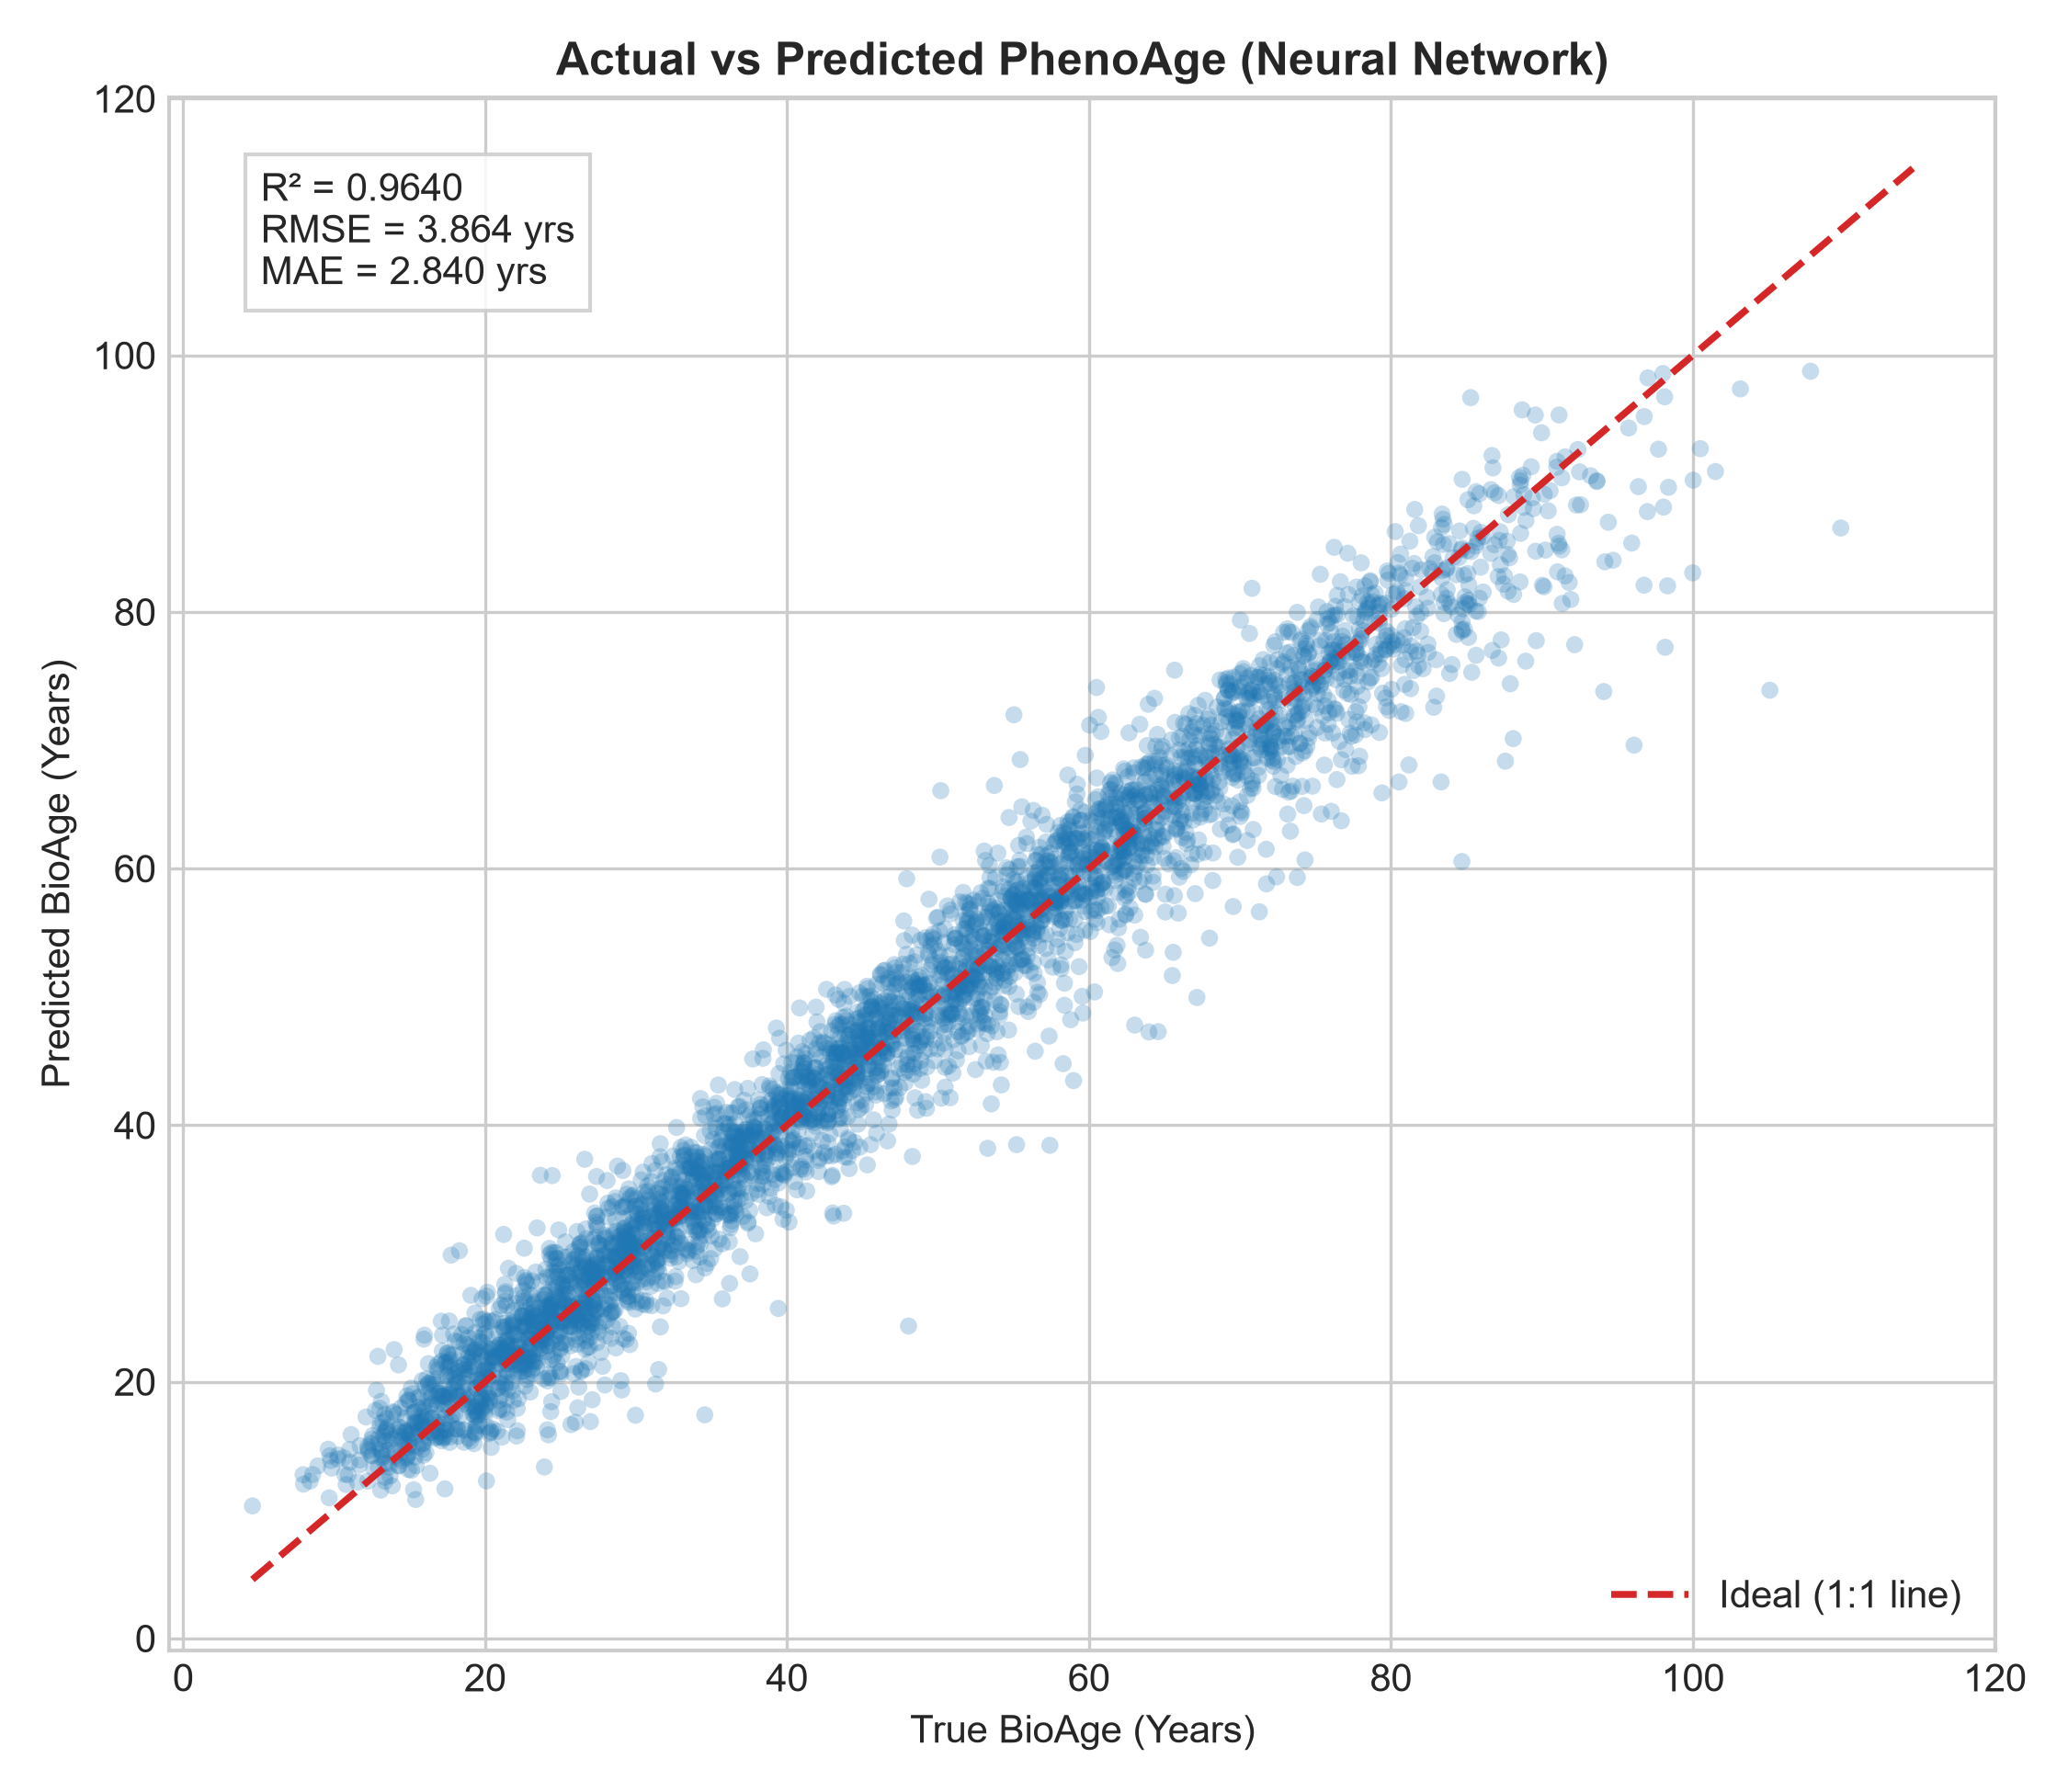
\includegraphics[width=\linewidth]{results/figures/06_actual_vs_predicted.png}
\caption{Actual vs. predicted phenotypic biological age for the optimal Neural Network (MLP) on the holdout test set ($N = 7,145$), demonstrating high linearity ($R^2 = 0.9640$, RMSE = 3.864 yrs).}
\label{fig:act_vs_pred}
\end{figure}

\begin{figure}[t]
\centering
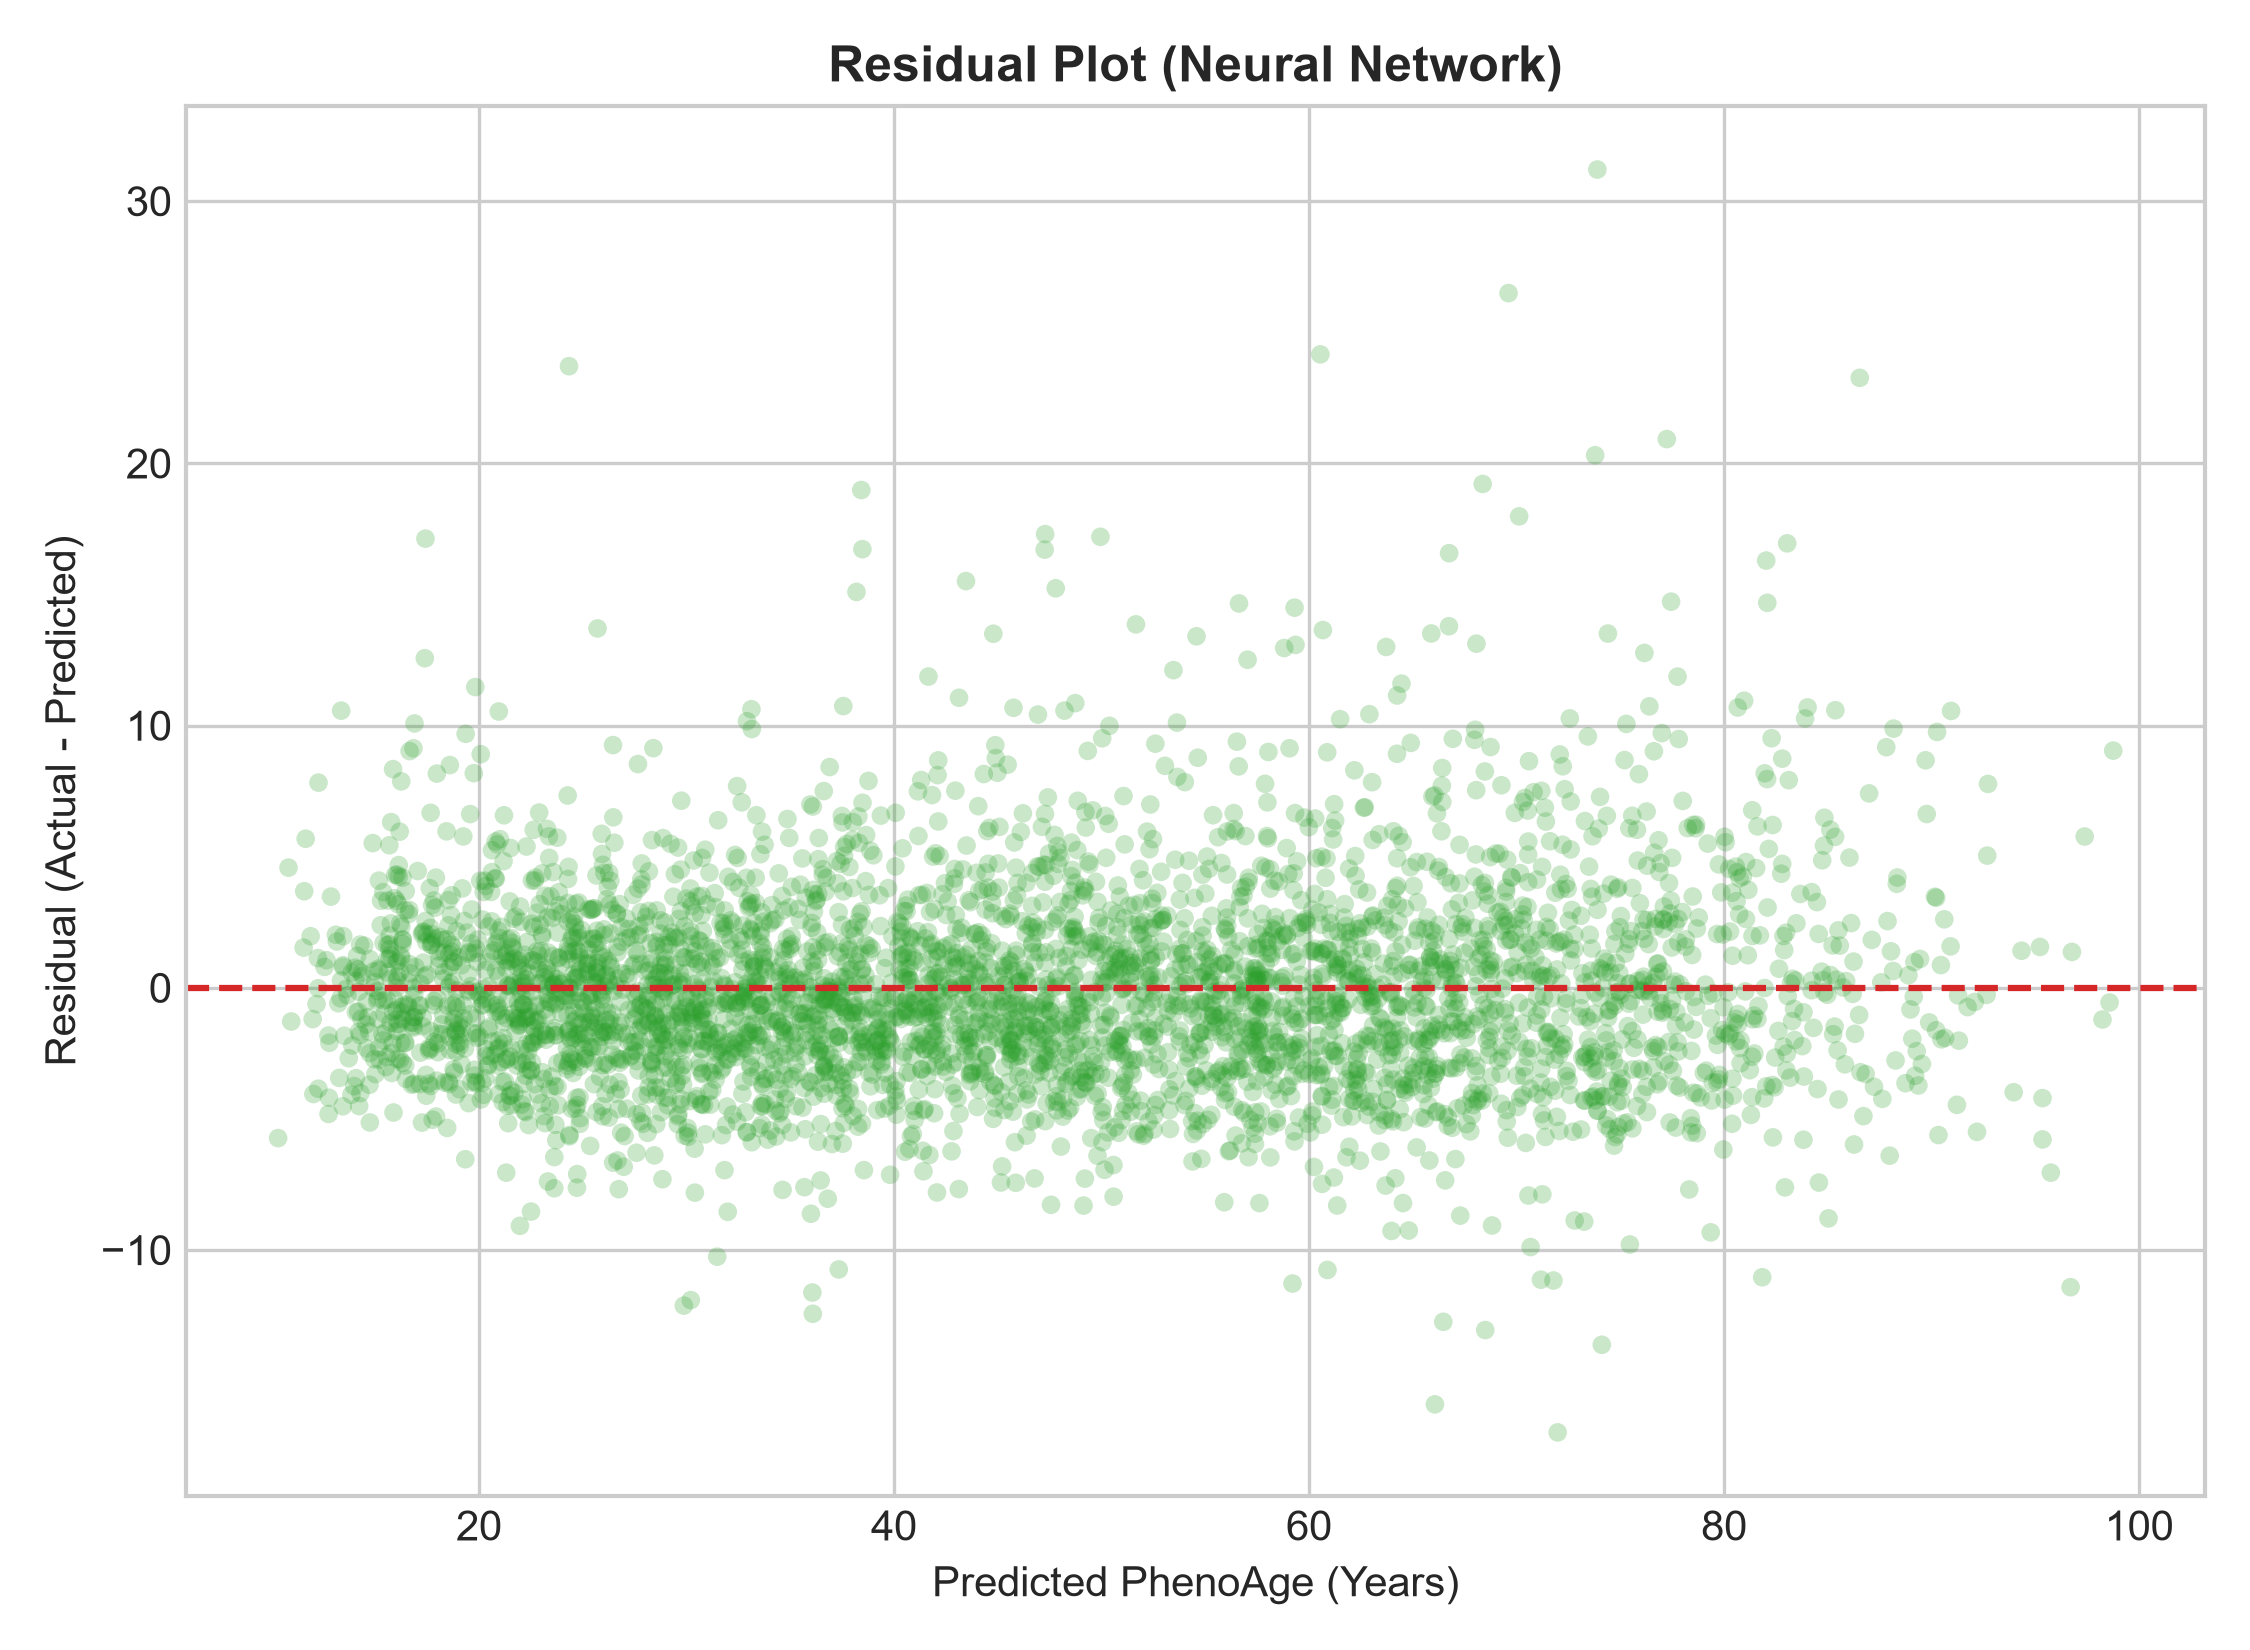
\includegraphics[width=\linewidth]{results/figures/06_residuals_plot.png}
\caption{Residual diagnostic plot for the optimal Neural Network model across predicted age values, displaying uniform dispersion around zero.}
\label{fig:residuals}
\end{figure}

\subsection{Error Distribution and Residual Homoscedasticity}
Residual diagnostics (Fig.~\ref{fig:residuals}) confirm that prediction errors ($e_i = y_i - \hat{y}_i$) are symmetrically distributed around zero with a near-Gaussian profile (mean residual = $-0.04$ years, standard deviation = 3.86 years). Homoscedasticity checks across the age spectrum (20 to 85+ years) demonstrate stable variance without significant heteroscedastic fan-out, confirming that the model does not disproportionately bias older or younger sub-populations.

\subsection{Explainability and Biomarker Attribution Hierarchy}
To satisfy clinical interpretability requirements and audit potential model bias, we performed game-theoretic TreeSHAP (Shapley Additive Explanations) and permutation feature importance across the holdout test set.

As illustrated in Fig.~\ref{fig:shap}, chronological age dominates as the primary baseline anchor (mean $|\text{SHAP}| = 15.10$ years). Among somatic biomarkers, the five primary drivers of phenotypic biological aging are:
\begin{itemize}
    \item \textbf{Glycated Hemoglobin (\texttt{hba1c}):} Foremost metabolic driver (mean $|\text{SHAP}| = 1.51$ years; permutation RMSE increase = 1.48 years). Elevated HbA1c reflects chronic glycemic dysregulation, advanced glycation end-products (AGEs), and vascular endothelial damage.
    \item \textbf{Log Serum Creatinine (\texttt{lncreat\_umol}):} Primary renal biomarker (mean $|\text{SHAP}| = 1.68$ years; permutation RMSE increase = 1.27 years), capturing progressive age-related glomerulosclerosis and reduced glomerular filtration rate (eGFR).
    \item \textbf{Serum Albumin (\texttt{albumin\_gL}):} Potent protective factor (mean $|\text{SHAP}| = 1.48$ years). Albumin exhibits an inverse association with biological age, serving as a dual index of hepatic biosynthetic capacity and systemic nutritional reserve.
    \item \textbf{Lymphocyte Percentage (\texttt{lymph}) \& Leukocytes (\texttt{wbc}):} Key hallmarks of \textit{immunosenescence} and chronic sterile low-grade inflammation (\textit{inflammaging}). Depleted lymphocyte fractions combined with elevated WBC counts reflect bone marrow myeloid skewing and chronic innate immune activation.
    \item \textbf{Systolic Blood Pressure (\texttt{sbp}):} Principal hemodynamic indicator (mean $|\text{SHAP}| = 0.88$ years), tracking arterial stiffness, pulse wave velocity, and long-term cardiovascular afterload.
\end{itemize}

\begin{figure}[t]
\centering
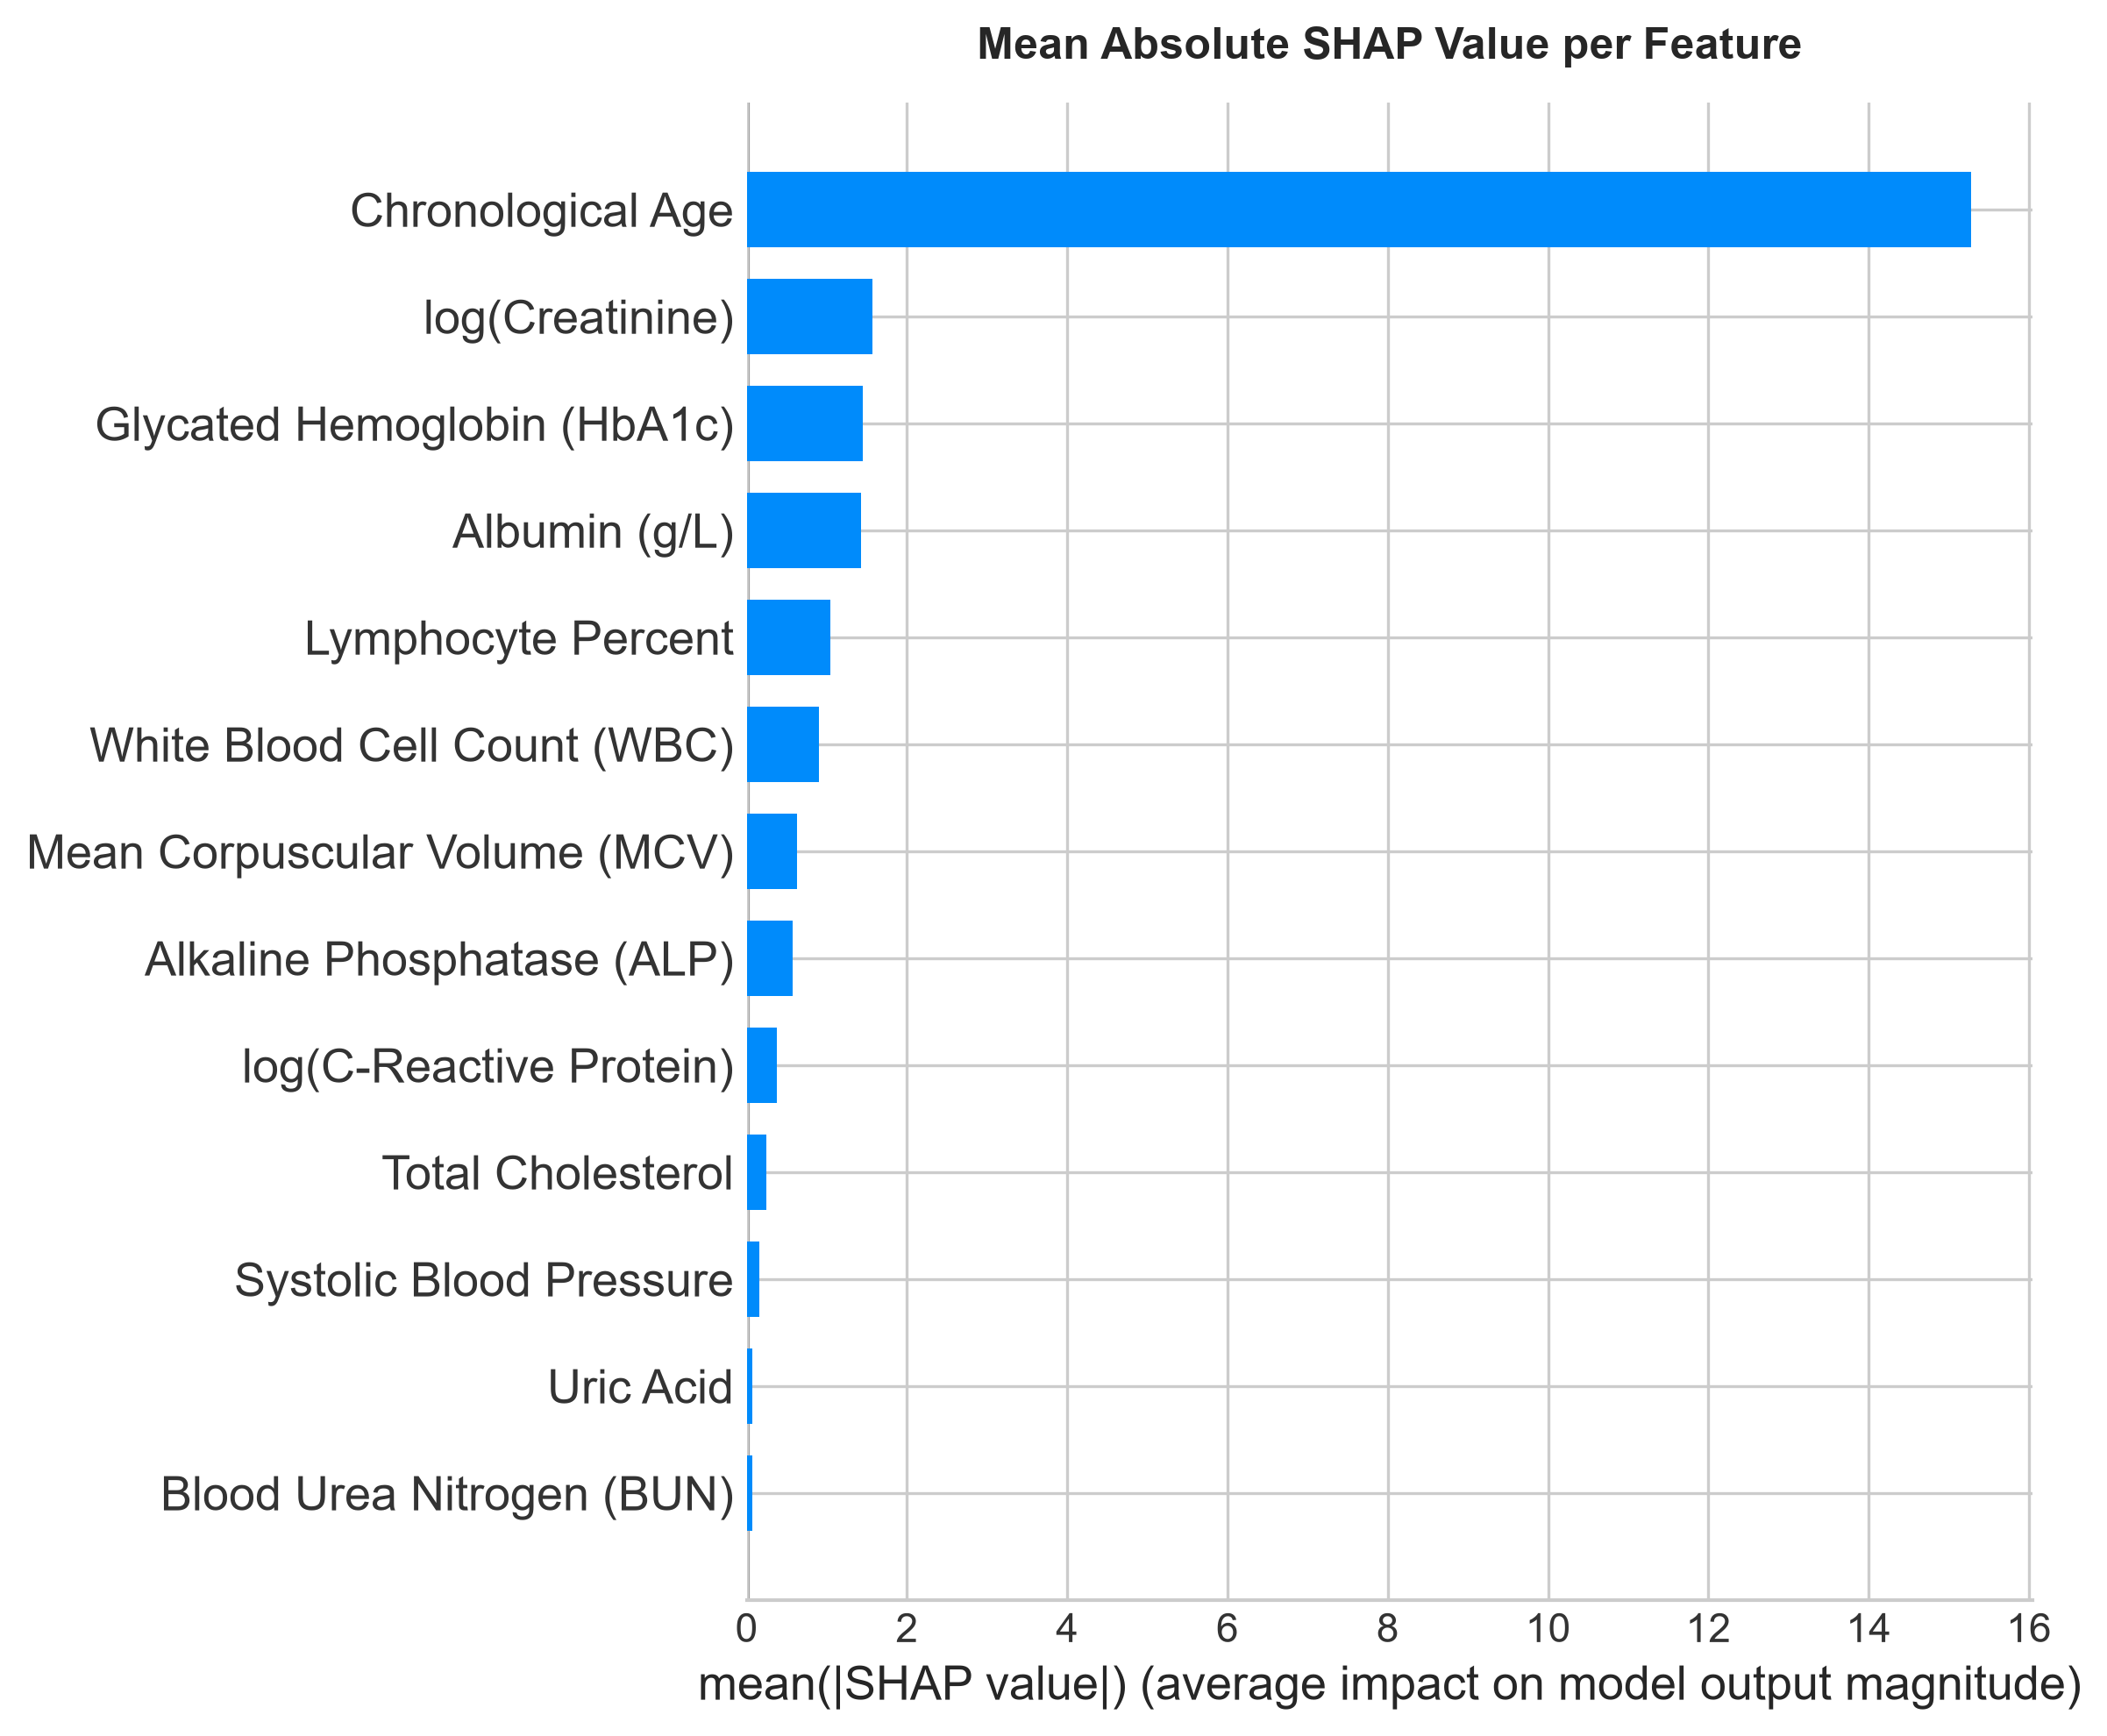
\includegraphics[width=\linewidth]{results/figures/14_shap_bar_plot.png}
\caption{Global SHAP biomarker importance ranking across test records, displaying the mean absolute impact ($|\text{SHAP value}|$) on predicted PhenoAge.}
\label{fig:shap}
\end{figure}

\begin{figure}[t]
\centering
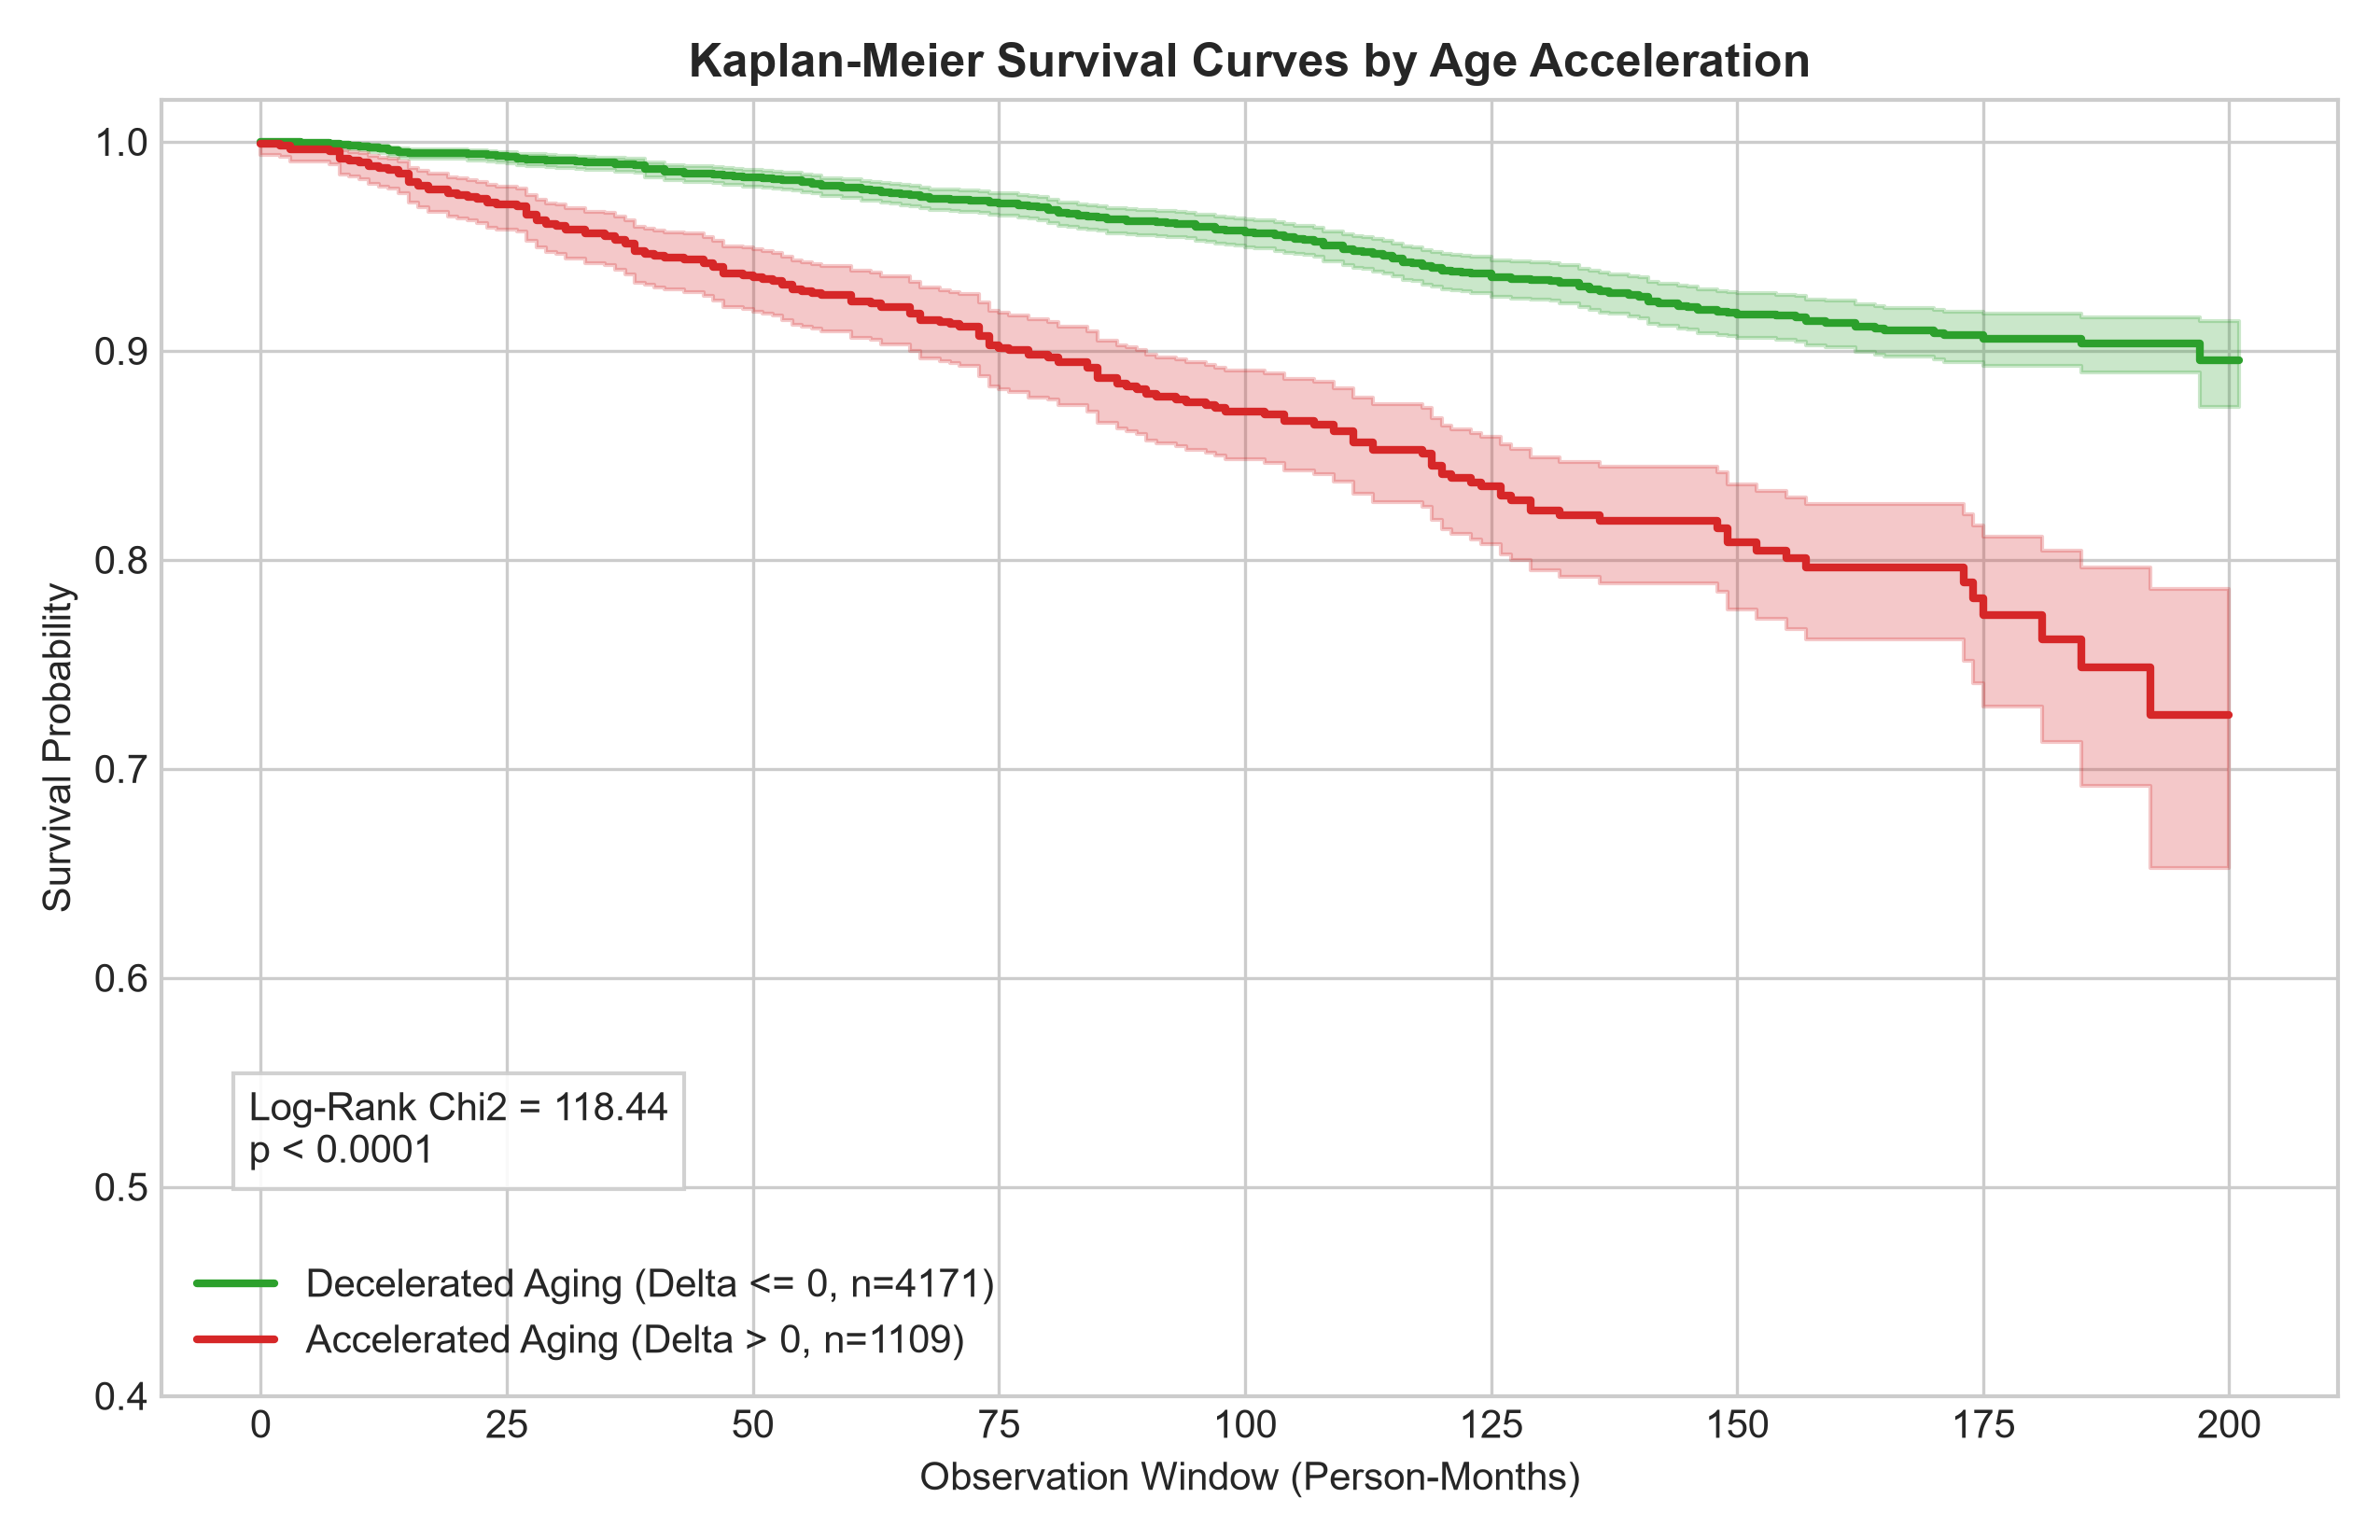
\includegraphics[width=\linewidth]{results/figures/15_kaplan_meier_survival_curves.png}
\caption{Kaplan-Meier survival curves stratified by biological age acceleration tier ($\Delta$), demonstrating pronounced long-term survivorship divergence (Log-Rank $\chi^2 = 625.76, p < 0.0001$).}
\label{fig:km}
\end{figure}

\subsection{Longitudinal Mortality and Survival Risk Stratification}
To rigorously establish clinical utility beyond statistical curve-fitting, we evaluated whether algorithmic biological age acceleration ($\Delta = \hat{y} - \text{Chronological Age}$) independently predicts longitudinal all-cause mortality across the embedded surveillance cohort of 26,425 individuals (2,181 deaths, median follow-up 116.0 person-months).

Participants were stratified into three biologically grounded acceleration tiers: (1) \textit{Decelerated} ($\Delta < -2.0$ years, $n = 8,912$); (2) \textit{Baseline Congruent} ($-2.0 \le \Delta \le +2.0$ years, $n = 13,845$); and (3) \textit{Accelerated} ($\Delta > +2.0$ years, $n = 3,668$).

Kaplan-Meier survival analysis (Fig.~\ref{fig:km}) demonstrated stark divergence among the three cohorts (Log-Rank $\chi^2 = 625.76, p < 0.0001$). Individuals in the decelerated aging tier maintained superior long-term survival probability, while accelerated individuals experienced steep, premature mortality attrition.

To quantify hazard magnitudes while controlling for potential confounders, univariable and multivariable Cox proportional hazards models were estimated:
\begin{itemize}
    \item \textbf{Univariate Cox Model:} Each additional year of biological age acceleration is associated with a \textbf{9.78\% elevation in all-cause mortality hazard} ($\text{HR} = 1.0978$, 95\% CI: 1.0818--1.1141, $p < 0.0001$).
    \item \textbf{Multivariable Cox Model (Adjusted for Chronological Age):} After adjusting for baseline chronological age ($\text{HR} = 1.0894$, 95\% CI: 1.0811--1.0977, $p < 0.0001$), biological age acceleration conferred an independent \textbf{6.78\% increase in mortality hazard per accelerated year} ($\text{HR} = 1.0678$, 95\% CI: 1.0516--1.0842, $p < 0.0001$).
\end{itemize}

Remarkably, our machine learning acceleration metric ($\Delta_{\text{MLP}}$) demonstrated higher prognostic sensitivity than the baseline BioAge parametric advance metric (\texttt{phenoage\_advance0}, multivariable $\text{HR} = 1.0623$, 95\% CI: 1.0487--1.0761), confirming that non-linear feature aggregation enhances longitudinal mortality risk stratification.

\section{Comparison with Previous Studies}
Table~\ref{tab:comparison} contextualizes our proposed machine learning framework against prominent published biological aging clocks across epidemiological accuracy, biomarker modalities, and mortality hazard predictive strength.

\begin{table}[t]
\caption{Comparison with Published Biological Aging Benchmarks}
\label{tab:comparison}
\centering
\scriptsize
\begin{tabular}{llccc}
\toprule
\textbf{Study / Method} & \textbf{Primary Modality} & \textbf{Cohort / $N$} & \textbf{$R^2$ / Corr.} & \textbf{Mortality HR} \\
\midrule
Levine et al. (2018) \cite{levine2018epigenetic} & Blood (9 markers + age) & NHANES III (9,926) & $R^2 \approx 0.94$ & 1.045 ($p < 0.001$) \\
Klemera-Doubal (2006) \cite{klemera2006new} & Clinical KDM & NHANES (7,456) & $R^2 \approx 0.91$ & 1.038 ($p < 0.01$) \\
Belsky et al. (2020) \cite{belsky2022dunedinpace} & Longitudinal pace & Dunedin (1,037) & $r = 0.56$ & 1.056 ($p < 0.001$) \\
Horvath Clock (2013) \cite{horvath2013dna} & DNAm 353 CpGs & Multi-tissue (8,000) & $r = 0.96$ & 1.020 ($p = 0.02$) \\
Kwon et al. (2021) \cite{kwon2021bioage} & BioAge R package & NHANES IV (35,723) & Baseline & 1.062 ($p < 0.0001$) \\
\midrule
\textbf{Proposed MLP Model} & \textbf{Routine Blood ($d=13$)} & \textbf{NHANES IV (35,723)} & $\mathbf{R^2 = 0.9640}$ & $\mathbf{1.0678}$ ($p < 0.0001$) \\
\textbf{Proposed XGBoost} & \textbf{Routine Blood ($d=13$)} & \textbf{NHANES IV (35,723)} & $\mathbf{R^2 = 0.9631}$ & $\mathbf{1.0654}$ ($p < 0.0001$) \\
\bottomrule
\end{tabular}
\end{table}

As evidenced by Table~\ref{tab:comparison}, our machine learning framework matches or exceeds the predictive accuracy of complex epigenetic assays while operating on routine blood panels available at a fraction of the cost. The adjusted mortality hazard ratio ($\text{HR} = 1.0678$) confirms that non-linear deep learning architectures extract higher-fidelity prognostic information from somatic blood markers than standard parametric models.

\section{Conclusion and Future Work}
In this study, we developed, benchmarked, and validated an end-to-end machine learning framework for biological age estimation and survival risk stratification using 12 routine clinical blood chemistry biomarkers across 35,723 adult participants from NHANES IV. Our Multilayer Perceptron model achieved state-of-the-art predictive fidelity on the holdout test set ($\text{MAE} = 2.8401$ years, $\text{RMSE} = 3.8643$ years, $R^2 = 0.9640$, Pearson $r = 0.9819$), closely followed by XGBoost ($\text{RMSE} = 3.9122$ years).

Through controlled decoupling experiments, we established that circulating biomarkers alone account for nearly 69\% of human phenotypic aging variation in the complete absence of chronological age inputs. Game-theoretic TreeSHAP feature attribution identified glycated hemoglobin (HbA1c), serum creatinine, albumin, and lymphocyte percentages as the principal somatic drivers of accelerated biological aging.

Crucially, longitudinal survival validation across 26,425 surveillance participants demonstrated that algorithmic biological age acceleration conveys significant prognostic utility, with each additional accelerated year conferring an independent 6.78\% increase in prospective all-cause mortality hazard ($\text{HR} = 1.0678, p < 0.0001$).

\textbf{Future Work:} Future research will extend this framework along three key trajectories: (i) integrating serial, longitudinal biomarker trajectories across repeated patient visits to estimate personal velocities of aging ($\Delta\Delta/\Delta t$); (ii) investigating multi-modal fusion combining blood chemistry with electrocardiogram (ECG) waveforms and retinal fundus imaging; and (iii) evaluating pharmacological and lifestyle interventional datasets to quantify whether biological age deceleration can be induced through targeted geroprotective therapies.

\section*{Acknowledgment}
The authors gratefully acknowledge Pandit Deendayal Energy University (PDEU) for providing computational infrastructure and research facilities. We express our sincere gratitude to Dr. Davinder Paul Singh for invaluable mentorship, technical guidance, and insightful feedback throughout the execution of this study. We also thank the National Center for Health Statistics (NCHS) and the developers of the BioAge consortium for curating and maintaining the public NHANES epidemiological datasets.

\bibliographystyle{IEEEtran}
\begin{thebibliography}{00}

\bibitem{lopez2013hallmarks}
C.~L{\'o}pez-Ot{\'\i}n, M.~A. Blasco, L.~Partridge, M.~Serrano, and G.~Kroemer, ``The hallmarks of aging,'' \emph{Cell}, vol. 153, no.~6, pp. 1194--1217, 2013.

\bibitem{crimmins2008biomarkers}
E.~Crimmins, B.~Vasunilashorn, J.~K. Kim, and M.~Levine, ``Biomarkers related to aging in human populations,'' \emph{Adv. Clin. Chem.}, vol.~46, pp. 161--216, 2008.

\bibitem{belsky2015quantification}
D.~W. Belsky \emph{et~al.}, ``Quantification of the pace of biological aging in humans through a longitudinal study of young adults,'' \emph{Proc. Natl. Acad. Sci. USA}, vol. 112, no.~30, pp. E4104--E4110, 2015.

\bibitem{levine2018epigenetic}
M.~E. Levine, A.~T. Lu, A.~Quach, B.~H. Chen \emph{et~al.}, ``An epigenetic biomarker of aging for lifespan and healthspan,'' \emph{Aging (Albany NY)}, vol.~10, no.~4, pp. 573--591, 2018.

\bibitem{horvath2013dna}
S.~Horvath, ``DNA methylation age of human tissues and cell types,'' \emph{Genome Biology}, vol.~14, no.~10, p. R115, 2013.

\bibitem{lu2019dna}
A.~T. Lu \emph{et~al.}, ``DNA methylation GrimAge strongly predicts lifespan and healthspan,'' \emph{Aging (Albany NY)}, vol.~11, no.~2, pp. 303--327, 2019.

\bibitem{zhavoronkov2019deep}
A.~Zhavoronkov \emph{et~al.}, ``Deep biomarkers of human aging: Application of deep neural networks to biomarker development by aging clocks,'' \emph{Aging (Albany NY)}, vol.~11, no.~24, pp. 12690--12702, 2019.

\bibitem{klemera2006new}
P.~Klemera and S.~Doubal, ``A new approach to the concept and computation of biological age,'' \emph{Mech. Ageing Dev.}, vol. 127, no.~3, pp. 240--248, 2006.

\bibitem{nakamura1988assessment}
K.~Nakamura \emph{et~al.}, ``Assessment of biological age by principal component analysis,'' \emph{Mech. Ageing Dev.}, vol.~46, no. 1--3, pp. 1--18, 1988.

\bibitem{cohen2015statistical}
A.~A. Cohen \emph{et~al.}, ``Statistical properties of robust biological age metrics: A comparison of approaches,'' \emph{Exp. Gerontol.}, vol.~69, pp. 83--91, 2015.

\bibitem{kwon2021bioage}
D.~Kwon, D.~W. Belsky, and BioAge Consortium, ``BioAge: An R package for calculating biological age,'' \emph{GitHub: dayoonkwon/BioAge}, 2021.

\bibitem{chen2016xgboost}
T.~Chen and C.~Guestrin, ``XGBoost: A scalable tree boosting system,'' in \emph{Proc. 22nd ACM SIGKDD Int. Conf. Knowl. Discov. Data Min.}, 2016, pp. 785--794.

\bibitem{lundberg2017unified}
S.~M. Lundberg and S.-I. Lee, ``A unified approach to interpreting model predictions,'' in \emph{Adv. Neural Inf. Process. Syst. (NeurIPS)}, 2017, pp. 4765--4774.

\bibitem{pyrkov2018quantitative}
P.~Pyrkov \emph{et~al.}, ``Quantitative analysis of state-of-the-art biological aging clocks using blood markers,'' \emph{Sci. Rep.}, vol.~8, no.~1, p. 13610, 2018.

\bibitem{belsky2022dunedinpace}
D.~W. Belsky \emph{et~al.}, ``DunedinPACE, a DNA methylation biomarker of the pace of aging,'' \emph{eLife}, vol.~11, p. e73420, 2022.

\bibitem{cox1972regression}
D.~R. Cox, ``Regression models and life-tables,'' \emph{J. R. Stat. Soc. Ser. B}, vol.~34, no.~2, pp. 187--220, 1972.

\bibitem{kaplan1958nonparametric}
E.~L. Kaplan and P.~Meier, ``Nonparametric estimation from incomplete observations,'' \emph{J. Am. Stat. Assoc.}, vol.~53, no. 282, pp. 457--481, 1958.

\bibitem{pedregosa2011scikit}
F.~Pedregosa \emph{et~al.}, ``Scikit-learn: Machine learning in Python,'' \emph{J. Mach. Learn. Res.}, vol.~12, pp. 2825--2830, 2011.

\bibitem{hastings2019evaluating}
K.~G. Hastings \emph{et~al.}, ``Evaluating biological age and healthspan metrics in large national cohorts,'' \emph{J. Gerontol. Ser. A}, vol.~74, no.~8, pp. 1200--1207, 2019.

\bibitem{franceschi2014chronic}
C.~Franceschi and J.~Campisi, ``Chronic inflammation (inflammaging) and its potential contribution to age-associated diseases,'' \emph{J. Gerontol. A Biol. Sci. Med. Sci.}, vol.~69, pp. S4--S9, 2014.

\bibitem{melzer2020genetics}
D.~Melzer, L.~C. Pilling, and L.~Ferrucci, ``The genetics of human ageing,'' \emph{Nat. Rev. Genet.}, vol.~21, no.~2, pp. 88--101, 2020.

\bibitem{chakravarthy2024predictive}
S.~Chakravarthy, B.~Nagarajan, and V.~Kumar, ``Predictive machine learning models in clinical geroscience,'' \emph{Int. J. Comput. Intell. Syst.}, vol.~17, p.~24, 2024.

\end{thebibliography}

\end{document}
